\documentclass[11pt,a4paper]{article}

\usepackage[utf8]{inputenc}
\usepackage[T1]{fontenc}
\usepackage[spanish]{babel}
\usepackage[margin=2.4cm]{geometry}
\usepackage{graphicx}
\usepackage{booktabs}
\usepackage{amsmath}
\usepackage{amssymb}
\usepackage{float}
\usepackage{xcolor}
\usepackage{hyperref}

\hypersetup{
    colorlinks=true,
    linkcolor=blue!60!black,
    urlcolor=blue!60!black,
    citecolor=blue!60!black
}

\begin{document}

% ============================================================================
% PORTADA INSTITUCIONAL
% ============================================================================
\begin{titlepage}
    \centering
    \vspace*{0.8cm}

    % Descomentar la siguiente línea si se desea incluir el logotipo institucional:
    % \includegraphics[width=0.28\textwidth]{figuras/logo_universidad.png}\\[0.8cm]

    {\LARGE \textbf{\textcolor{blue!50!black}{NOMBRE DE LA UNIVERSIDAD / INSTITUCIÓN}}}\\[0.35cm]
    {\large \textsc{Maestría en Ciencia de Datos / Inteligencia Artificial}}\\[0.2cm]
    {\normalsize Asignatura: Prácticas de Estadística Aplicada}\\[1.6cm]

    \rule{\textwidth}{1.5pt}\\[0.5cm]
    {\LARGE \textbf{Predicción del Valor de Propiedades Inmobiliarias Basado en Características del Mercado y el Entorno}}\\[0.35cm]
    {\large Informe Técnico --- Proyecto Final (Caso 2)}\\[0.35cm]
    \rule{\textwidth}{1.5pt}\\[1.8cm]

    \begin{flushleft}
    \large
    \textbf{Presenta:} Nombre Completo del Estudiante \\[0.35cm]
    \textbf{Matrícula / ID:} 00000000 \\[0.35cm]
    \textbf{Docente:} Nombre del Profesor(a) \\[0.35cm]
    \textbf{Entregable:} Informe Técnico, Modelo de Regresión Lineal y Dashboard en Streamlit \\[0.35cm]
    \textbf{Repositorio / App:} \texttt{estadistica\_prediccion\_costo\_casa}
    \end{flushleft}

    \vfill

    {\large Ciudad, País}\\[0.2cm]
    {\large \today}
\end{titlepage}

\thispagestyle{plain}
\begin{abstract}
El presente informe documenta el desarrollo integral de un modelo predictivo para estimar el precio de propiedades residenciales en Estados Unidos a partir del conjunto de datos inmobiliarios \texttt{realtor-data.zip.csv} (2{,}226{,}382 registros originales). Tras un proceso riguroso de limpieza y filtrado de valores atípicos extremos, se conservaron 1{,}294{,}939 propiedades válidas distribuidas en 53 estados y territorios. Se realizó un análisis exploratorio y de correlación de Pearson, identificando a la superficie construida ($r = 0.5006$) y al número de baños ($r = 0.4979$) como los factores numéricos más influyentes en el precio. Posteriormente, se construyó un modelo estadístico de Regresión Lineal Múltiple con \texttt{scikit-learn}, demostrando que incorporar la ubicación geográfica (\texttt{state}) eleva el coeficiente de determinación $R^2$ de $0.2836$ a $0.5275$ y reduce el RMSE de \$282{,}102 a \$229{,}110 USD. Finalmente, se comparó la regresión lineal frente a algoritmos de Machine Learning (Ridge, Árbol de Decisión y \texttt{HistGradientBoostingRegressor}, que alcanzó $R^2 = 0.5742$), y se implementó una aplicación interactiva en Streamlit con un simulador de precios basado en Regresión Lineal listo para despliegue.
\end{abstract}

\tableofcontents
\newpage

\section{Introducción y Objetivos}

La valoración precisa de propiedades residenciales es un problema central en el sector inmobiliario, financiero y de planificación urbana. El precio de una vivienda responde simultáneamente a sus atributos físicos (superficie construida, habitaciones, baños, tamaño del terreno) y a factores externos o geográficos asociados al mercado local.

De acuerdo con los requerimientos del proyecto (\textit{Caso 2}), se establecieron los siguientes objetivos:
\begin{enumerate}
    \item Identificar los factores más influyentes en los precios de las propiedades mediante estadística descriptiva y análisis de correlación.
    \item Desarrollar e interpretar modelos estadísticos de regresión lineal múltiple con \texttt{scikit-learn} para cuantificar la relación entre las variables predictoras y el precio.
    \item Entrenar y comparar algoritmos de Machine Learning frente al modelo lineal base.
    \item Evaluar el desempeño predictivo utilizando las métricas MSE, RMSE, MAE y $R^2$.
    \item Presentar los resultados y un simulador interactivo de cálculo de precios en una aplicación web desarrollada en \textbf{Streamlit}.
\end{enumerate}

\section{Recolección, Descripción y Limpieza de Datos}

\subsection{Descripción del Dataset}
Se utilizó el archivo \texttt{realtor-data.zip.csv} proveniente de portales inmobiliarios públicos (Kaggle / Realtor.com). El conjunto original contiene \textbf{2{,}226{,}382 filas} y \textbf{12 columnas}: \texttt{brokered\_by}, \texttt{status}, \texttt{price}, \texttt{bed}, \texttt{bath}, \texttt{acre\_lot}, \texttt{street}, \texttt{city}, \texttt{state}, \texttt{zip\_code}, \texttt{house\_size} y \texttt{prev\_sold\_date}.

Es importante señalar, respecto al alcance teórico del caso, que el dataset disponible proporciona información detallada de características físicas (\texttt{house\_size} en pies cuadrados, \texttt{bed}, \texttt{bath}, \texttt{acre\_lot}) y ubicación geográfica (\texttt{state}, \texttt{city}, \texttt{zip\_code}), mientras que no incluye directamente variables externas como accesibilidad a hospitales/escuelas o PIB per cápita. Por ello, la variable \texttt{state} actúa como un \textit{proxy} geográfico-económico que absorbe las diferencias estructurales entre mercados regionales.

\subsection{Limpieza y Preprocesamiento}
En la inspección inicial se detectaron valores faltantes sustanciales en las variables numéricas clave: \texttt{house\_size} (568{,}484 nulos), \texttt{bath} (511{,}771), \texttt{bed} (481{,}317), \texttt{acre\_lot} (325{,}589) y \texttt{price} (1{,}541), así como errores evidentes de captura (precios de \$0 o superiores a \$2{,}000 millones, viviendas con más de 400 habitaciones o superficies de $10^9\text{ ft}^2$).

Para garantizar la validez estadística del modelado residencial, se aplicaron las siguientes reglas de depuración en \texttt{train\_model.py}:
\begin{itemize}
    \item Selección de variables relevantes (\texttt{price}, \texttt{bed}, \texttt{bath}, \texttt{acre\_lot}, \texttt{house\_size}, \texttt{state}, \texttt{status}) y eliminación de registros con valores nulos (quedando 1{,}360{,}716 registros).
    \item Filtrado de rangos realistas para viviendas residenciales:
    \begin{itemize}
        \item Precio: $\$30{,}000 \le \texttt{price} \le \$2{,}000{,}000$ USD.
        \item Superficie construida: $400 \le \texttt{house\_size} \le 8{,}000\text{ ft}^2$ (aprox. $37$ a $743\text{ m}^2$).
        \item Habitaciones: $1 \le \texttt{bed} \le 10$; Baños: $1 \le \texttt{bath} \le 8$.
        \item Terreno: $0 < \texttt{acre\_lot} \le 20$ acres.
    \end{itemize}
    \item Exclusión de territorios con menos de 100 observaciones para estabilidad de las variables indicadoras por estado.
\end{itemize}

Tras el proceso de limpieza se obtuvieron \textbf{1{,}294{,}939 propiedades limpias} (58.16\% del total original) pertenecientes a \textbf{53 estados y territorios}, de las cuales 705{,}009 corresponden a viviendas en venta (\texttt{for\_sale}) y 589{,}930 a ventas cerradas (\texttt{sold}).

\section{Análisis Exploratorio de Datos (EDA)}

\subsection{Estadísticas Descriptivas}
La Tabla~\ref{tab:descriptivas} resume las medidas de tendencia central y dispersión del conjunto limpio. La mediana del precio es de \$369{,}900 USD, inferior a la media (\$455{,}929 USD), lo que evidencia una asimetría positiva típica de los mercados inmobiliarios. La vivienda típica cuenta con 3 habitaciones, 2 baños, 1{,}791 $\text{ft}^2$ ($\approx 166\text{ m}^2$) de construcción y un terreno de 0.21 acres ($\approx 850\text{ m}^2$).

\begin{table}[H]
\centering
\caption{Estadísticas descriptivas del conjunto de datos limpio ($N = 1{,}294{,}939$).}
\label{tab:descriptivas}
\resizebox{\textwidth}{!}{%
\begin{tabular}{lrrrrr}
\toprule
\textbf{Variable} & \textbf{Media} & \textbf{Desv. Est.} & \textbf{Mín.} & \textbf{Mediana} & \textbf{Máx.} \\
\midrule
Precio (USD) & 455{,}928.62 & 334{,}082.18 & 30{,}000 & 369{,}900 & 2{,}000{,}000 \\
Habitaciones (\texttt{bed}) & 3.33 & 0.99 & 1.00 & 3.00 & 10.00 \\
Baños (\texttt{bath}) & 2.45 & 0.99 & 1.00 & 2.00 & 8.00 \\
Terreno (\texttt{acre\_lot}) & 0.73 & 1.88 & 0.01 & 0.21 & 20.00 \\
Superficie (\texttt{house\_size}, $\text{ft}^2$) & 1{,}994.03 & 926.87 & 400.00 & 1{,}791.00 & 8{,}000.00 \\
\bottomrule
\end{tabular}%
}
\end{table}

La Figura~\ref{fig:distribuciones} muestra los histogramas de las variables principales y la transformación logarítmica del precio, la cual aproxima una distribución simétrica cercana a la normal.

\begin{figure}[H]
    \centering
    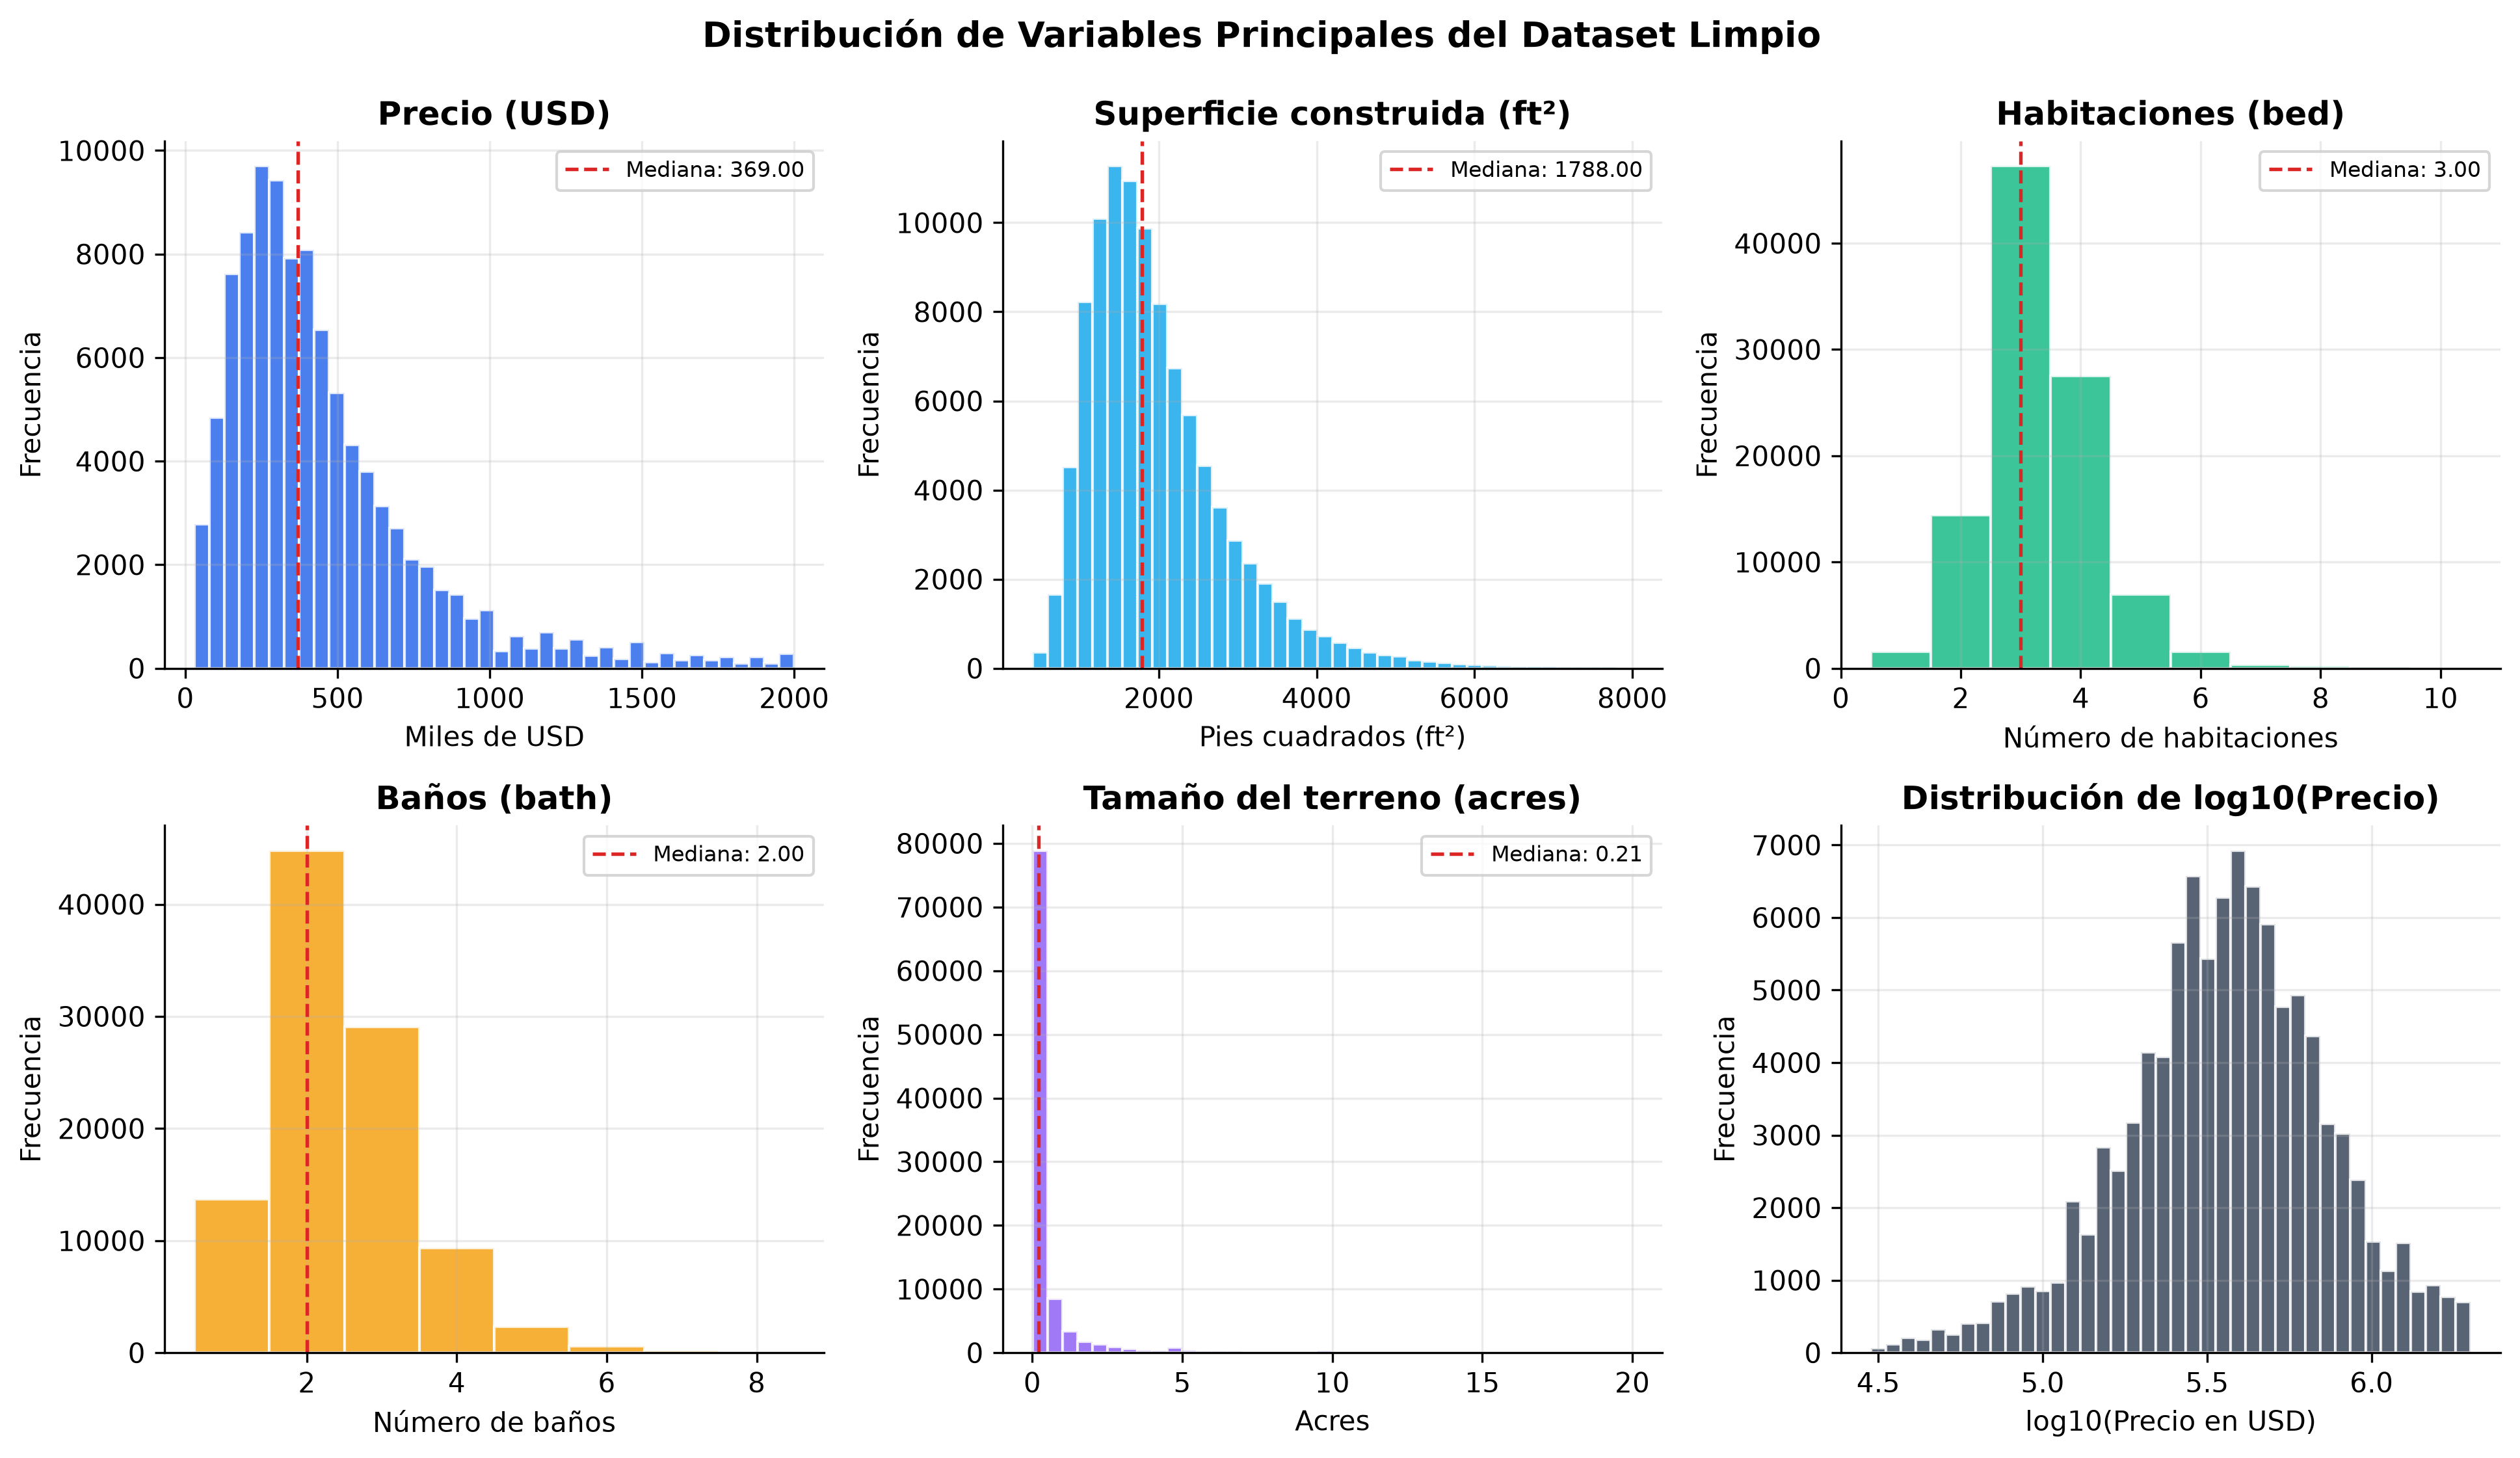
\includegraphics[width=0.96\textwidth]{figuras/distribuciones.png}
    \caption{Distribución de las variables numéricas principales en el dataset limpio.}
    \label{fig:distribuciones}
\end{figure}

\subsection{Análisis de Correlación}
La matriz de correlación de Pearson (Figura~\ref{fig:correlacion}) revela tres hallazgos fundamentales:
\begin{enumerate}
    \item \textbf{Predictores más fuertes:} \texttt{house\_size} ($r = 0.5006$) y \texttt{bath} ($r = 0.4979$) presentan la mayor correlación lineal positiva con el precio.
    \item \textbf{Multicolinealidad entre atributos estructurales:} Existe una correlación elevada entre \texttt{bath} y \texttt{house\_size} ($r = 0.7530$), así como entre \texttt{bed} y \texttt{house\_size} ($r = 0.6351$). Esto indica que las viviendas más grandes concentran simultáneamente más habitaciones y baños.
    \item \textbf{Baja correlación lineal del terreno:} \texttt{acre\_lot} muestra $r = 0.0748$ con el precio, debido a que terrenos extensos suelen ubicarse en zonas rurales de menor precio por metro cuadrado que lotes pequeños en áreas metropolitanas densas.
\end{enumerate}

\begin{figure}[H]
    \centering
    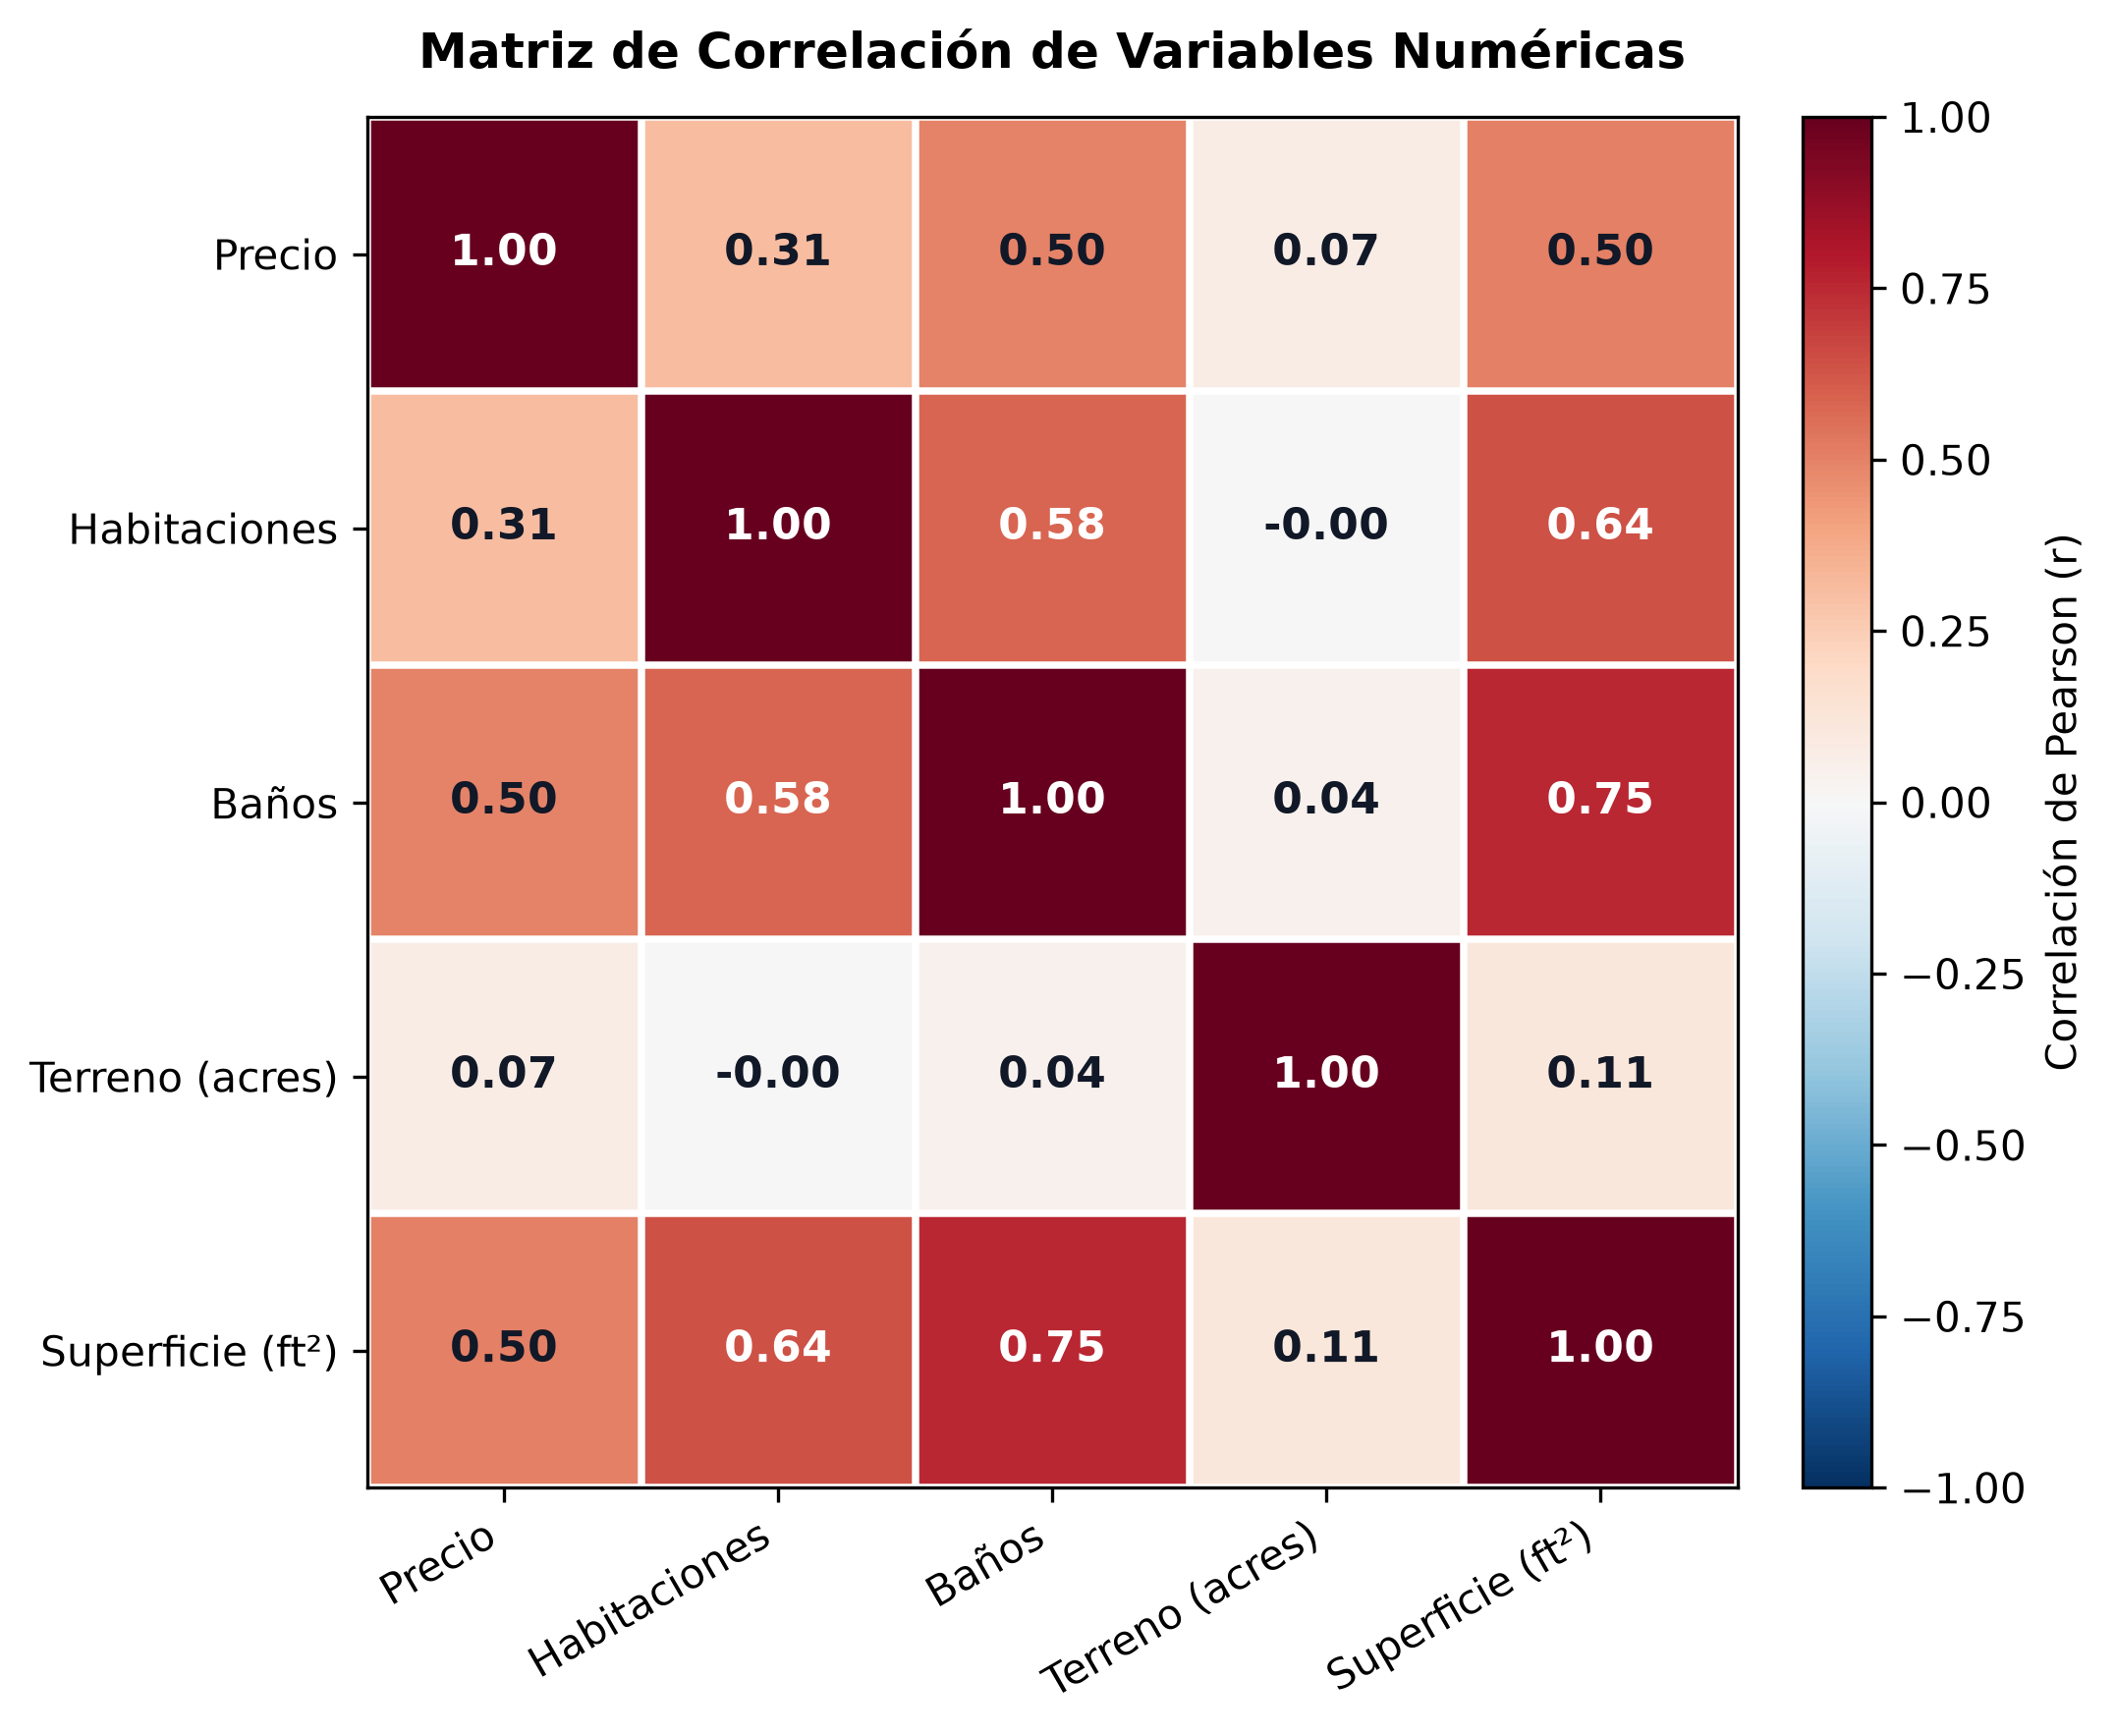
\includegraphics[width=0.68\textwidth]{figuras/correlacion.png}
    \caption{Matriz de correlación de Pearson entre las variables numéricas.}
    \label{fig:correlacion}
\end{figure}

\subsection{Heterogeneidad Geográfica}
El mercado inmobiliario estadounidense presenta diferencias regionales muy marcadas (Figura~\ref{fig:estados}). Mientras que el Distrito de Columbia (\$849{,}000), Hawái (\$730{,}000) y California (\$685{,}000) registran los precios medianos más elevados, estados como Puerto Rico (\$157{,}000), Ohio (\$179{,}000) y Virginia Occidental (\$209{,}000) presentan valores considerablemente menores para viviendas de tamaño comparable. Esto confirma que la ubicación es indispensable en el modelo predictivo.

\begin{figure}[H]
    \centering
    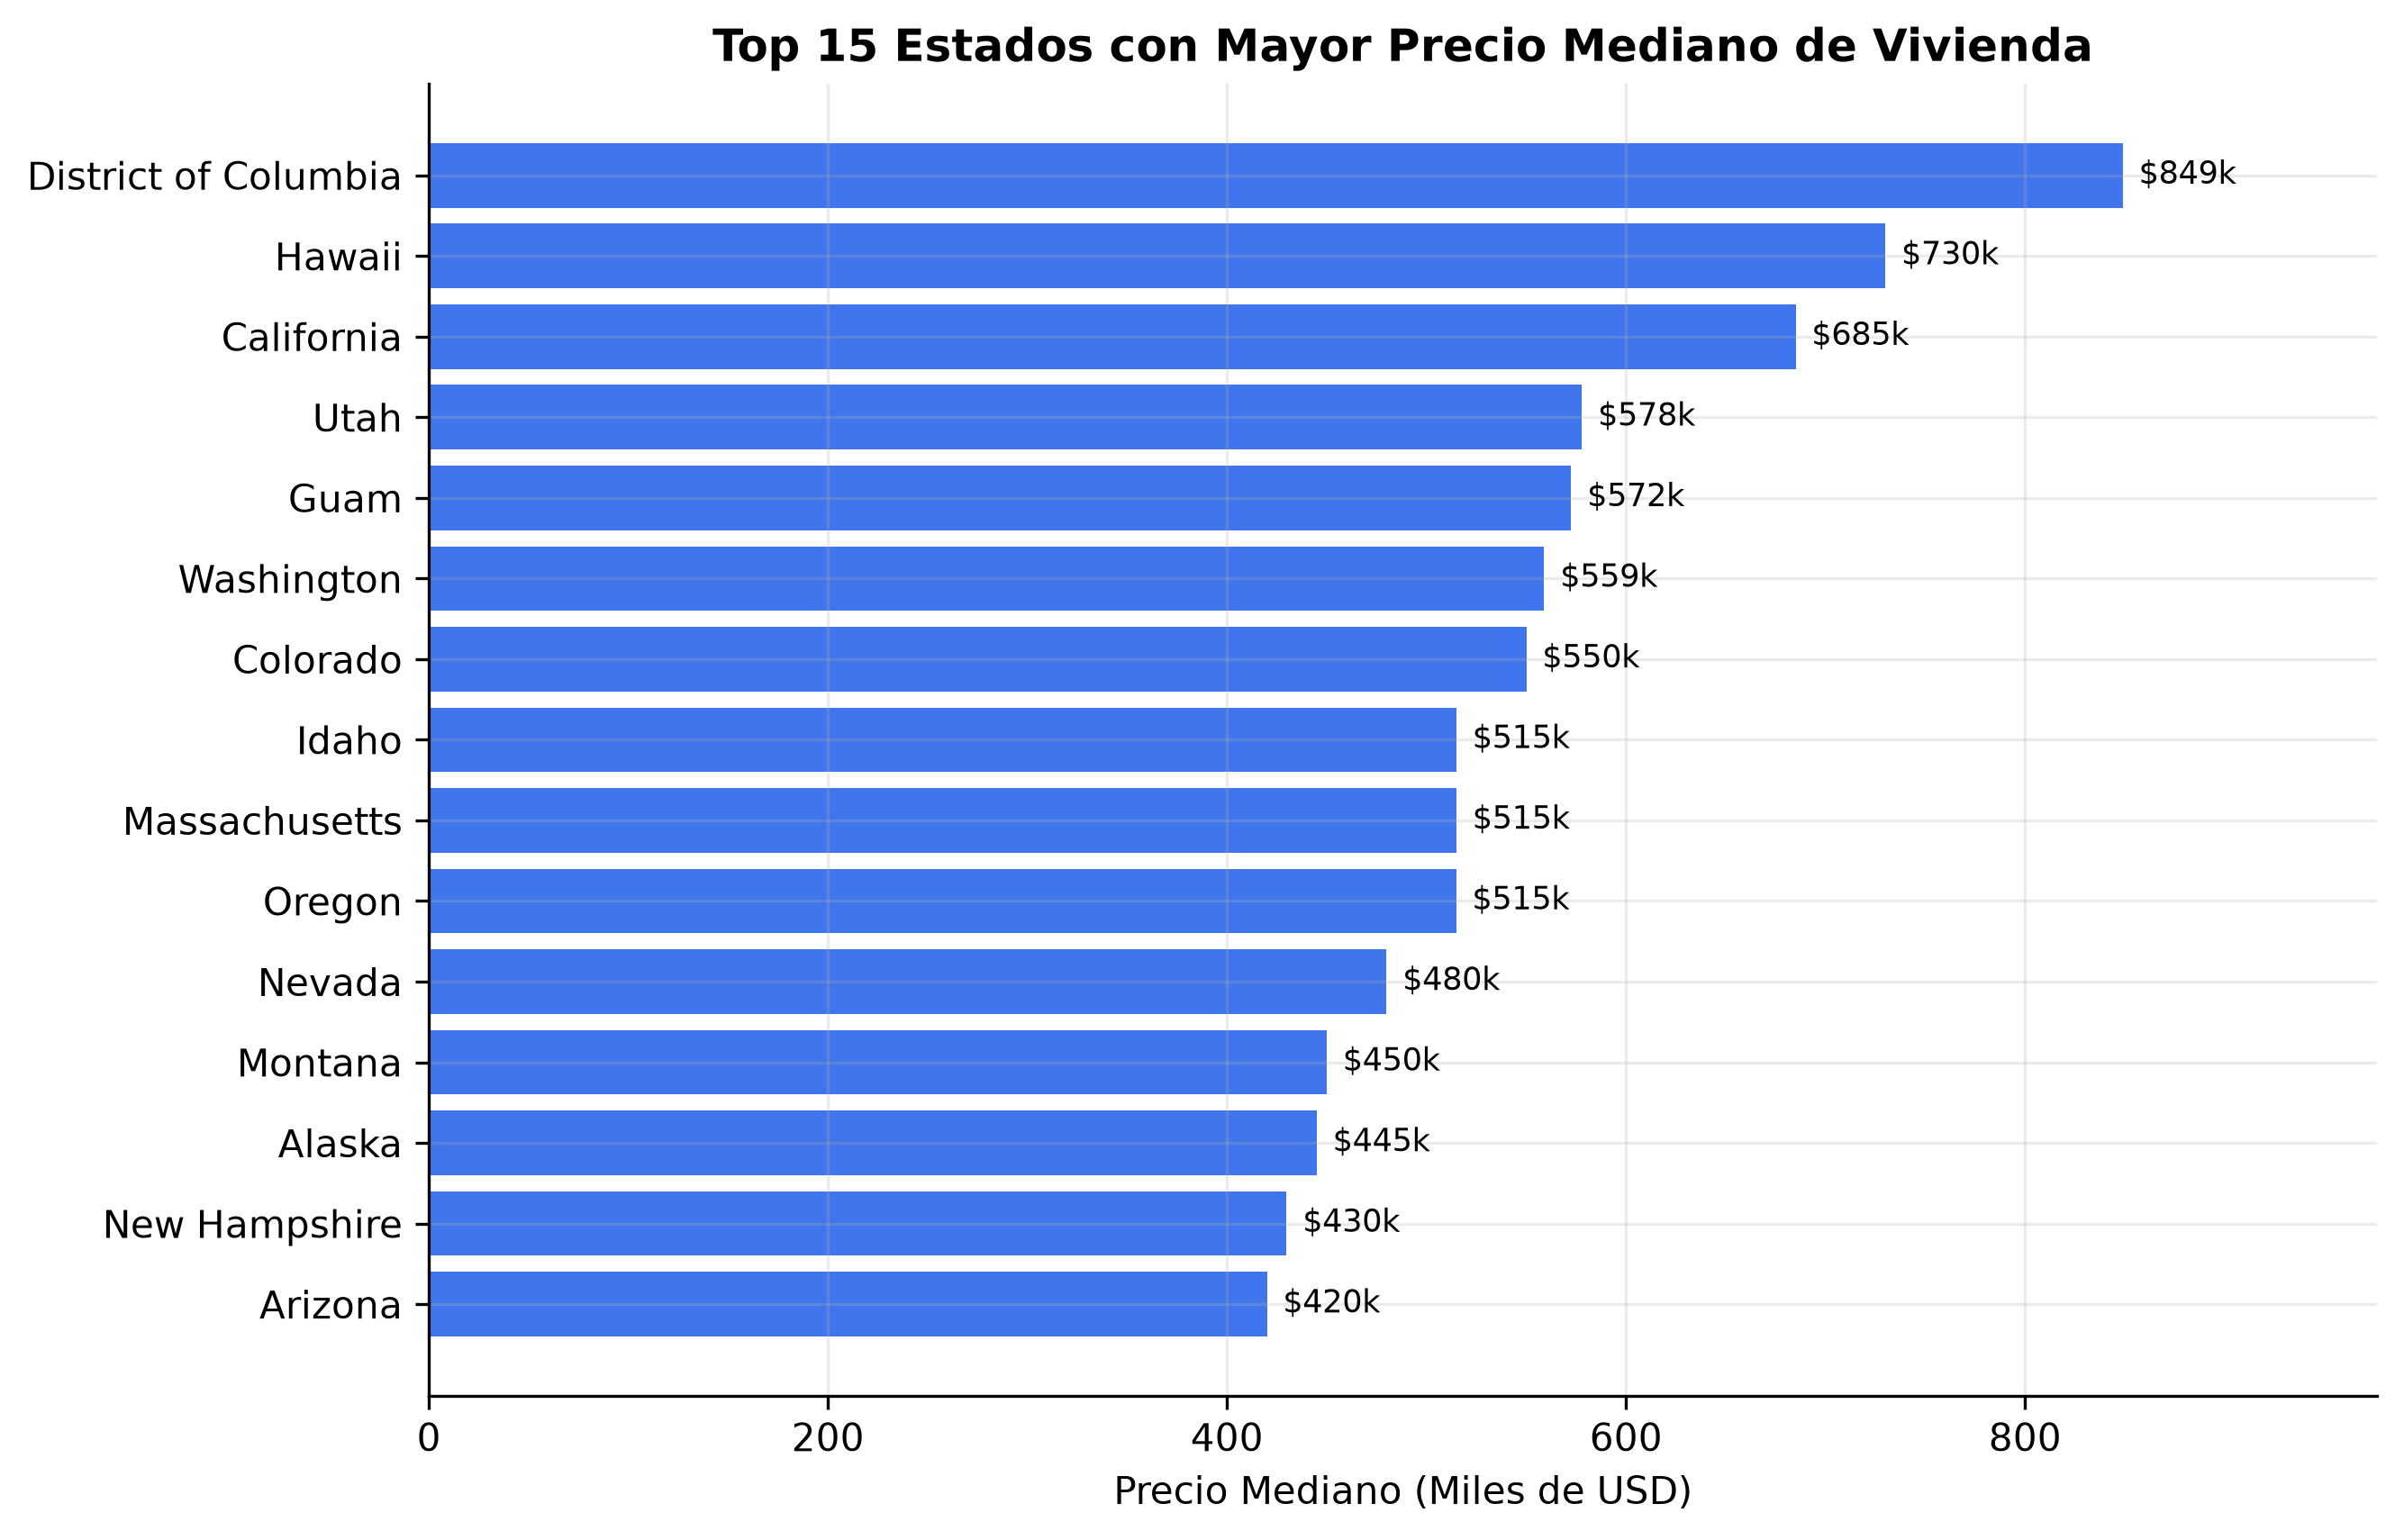
\includegraphics[width=0.84\textwidth]{figuras/top_estados.png}
    \caption{Top 15 estados y territorios con mayor precio mediano de vivienda.}
    \label{fig:estados}
\end{figure}

\section{Modelado Estadístico: Regresión Lineal Múltiple}

El conjunto limpio se dividió aleatoriamente en \textbf{80\% entrenamiento} (1{,}035{,}951 propiedades) y \textbf{20\% prueba} (258{,}988 propiedades) con semilla fija (\texttt{random\_state=42}).

\subsection{Especificación del Modelo}
Se ajustaron dos versiones del modelo de Regresión Lineal Ordinaria (\texttt{LinearRegression} de \texttt{scikit-learn}):
\begin{enumerate}
    \item \textbf{Modelo Base (Solo Numéricas):} Incluye únicamente \texttt{bed}, \texttt{bath}, \texttt{acre\_lot} y \texttt{house\_size}.
    \item \textbf{Modelo Principal (Numéricas + Estado):} Incorpora la variable categórica \texttt{state} mediante codificación \textit{One-Hot} (tomando \textit{Alabama} como categoría de referencia):
\end{enumerate}
\begin{equation}
\widehat{\text{Precio}} = \beta_0 + \beta_1 \cdot \text{bed} + \beta_2 \cdot \text{bath} + \beta_3 \cdot \text{acre\_lot} + \beta_4 \cdot \text{house\_size} + \sum_{k=1}^{52} \gamma_k \cdot \mathbb{I}(\text{state} = k)
\end{equation}

\subsection{Interpretación de Coeficientes}
La Tabla~\ref{tab:coeficientes} presenta los parámetros estimados del modelo principal de Regresión Lineal.

\begin{table}[H]
\centering
\caption{Coeficientes estimados de la Regresión Lineal Múltiple (Modelo Principal).}
\label{tab:coeficientes}
\resizebox{\textwidth}{!}{%
\begin{tabular}{lrp{7.8cm}}
\toprule
\textbf{Variable} & \textbf{Coeficiente (USD)} & \textbf{Interpretación (\textit{ceteris paribus})} \\
\midrule
Intercepto ($\beta_0$, base Alabama) & $-\$18{,}577.54$ & Constante de ajuste para el estado de referencia. \\
Superficie (\texttt{house\_size}, $\text{ft}^2$) & $+\$143.73$ & Cada pie cuadrado adicional incrementa el precio esperado en \$143.73 USD ($\approx \$1{,}547/\text{m}^2$). \\
Baños (\texttt{bath}) & $+\$83{,}779.48$ & Cada baño adicional aporta en promedio \$83{,}779 USD al valor de la propiedad. \\
Habitaciones (\texttt{bed}) & $-\$23{,}434.56$ & Efecto parcial negativo al mantener fija la superficie y los baños: dividir el mismo metraje en más cuartos pequeños reduce el valor percibido (efecto de multicolinealidad). \\
Terreno (\texttt{acre\_lot}, acres) & $+\$6{,}482.16$ & Cada acre adicional de terreno aporta \$6{,}482 USD. \\
\midrule
\multicolumn{3}{l}{\textit{Ejemplos de ajustes geográficos ($\gamma_k$ respecto a Alabama):}} \\
Hawaii & $+\$507{,}622.77$ & Prima regional más alta del país. \\
District of Columbia & $+\$427{,}159.46$ & Mercado urbano de alta densidad y demanda. \\
California & $+\$416{,}055.18$ & Fuerte prima por ubicación costera y económica. \\
Texas & $-\$35{,}037.24$ & Mercado más asequible a igualdad de superficie. \\
West Virginia & $-\$176{,}672.51$ & Menor valoración relativa en el conjunto analizado. \\
\bottomrule
\end{tabular}%
}
\end{table}

El signo negativo del coeficiente parcial de \texttt{bed} ($-\$23{,}434.56$) a pesar de su correlación bivariada positiva ($r = 0.3100$) es un fenómeno clásico de \textbf{multicolinealidad} en econometría inmobiliaria: al controlar por la superficie total (\texttt{house\_size}) y el número de baños (\texttt{bath}), incrementar únicamente el número de habitaciones implica habitaciones más reducidas dentro de la misma área construida.

\section{Modelado con Machine Learning y Comparación de Modelos}

Para cumplir con las fases de modelado predictivo y evaluación comparativa, se entrenaron tres algoritmos adicionales de Machine Learning sobre la misma partición de entrenamiento y prueba: \textbf{Regresión Ridge} (regularización L2 con estandarización), \textbf{Árbol de Decisión} (\texttt{max\_depth=14}) y \textbf{Gradient Boosting} (\texttt{HistGradientBoostingRegressor}).

\begin{table}[H]
\centering
\caption{Comparación de desempeño de los modelos en el conjunto de prueba ($N_{\text{test}} = 258{,}988$).}
\label{tab:modelos}
\resizebox{\textwidth}{!}{%
\begin{tabular}{llrrrr}
\toprule
\textbf{Modelo} & \textbf{Categoría} & \textbf{$R^2$} & \textbf{RMSE (USD)} & \textbf{MAE (USD)} & \textbf{MSE ($\times 10^9$)} \\
\midrule
Regresión Lineal (Solo Numéricas) & Estadístico & 0.2836 & 282{,}101.57 & 195{,}832.09 & 79.58 \\
\textbf{Regresión Lineal (+ Estado)} & \textbf{Estadístico (Principal)} & \textbf{0.5275} & \textbf{229{,}109.85} & \textbf{151{,}944.68} & \textbf{52.49} \\
Regresión Ridge (L2 + Estado) & Machine Learning & 0.5292 & 228{,}700.81 & 151{,}443.63 & 52.30 \\
Árbol de Decisión (\texttt{max\_depth=14}) & Machine Learning & 0.5346 & 227{,}381.83 & 149{,}555.07 & 51.70 \\
Gradient Boosting (\texttt{HistGBR}) & Machine Learning & \textbf{0.5742} & \textbf{217{,}496.75} & \textbf{141{,}119.92} & \textbf{47.30} \\
\bottomrule
\end{tabular}%
}
\end{table}

\begin{figure}[H]
    \centering
    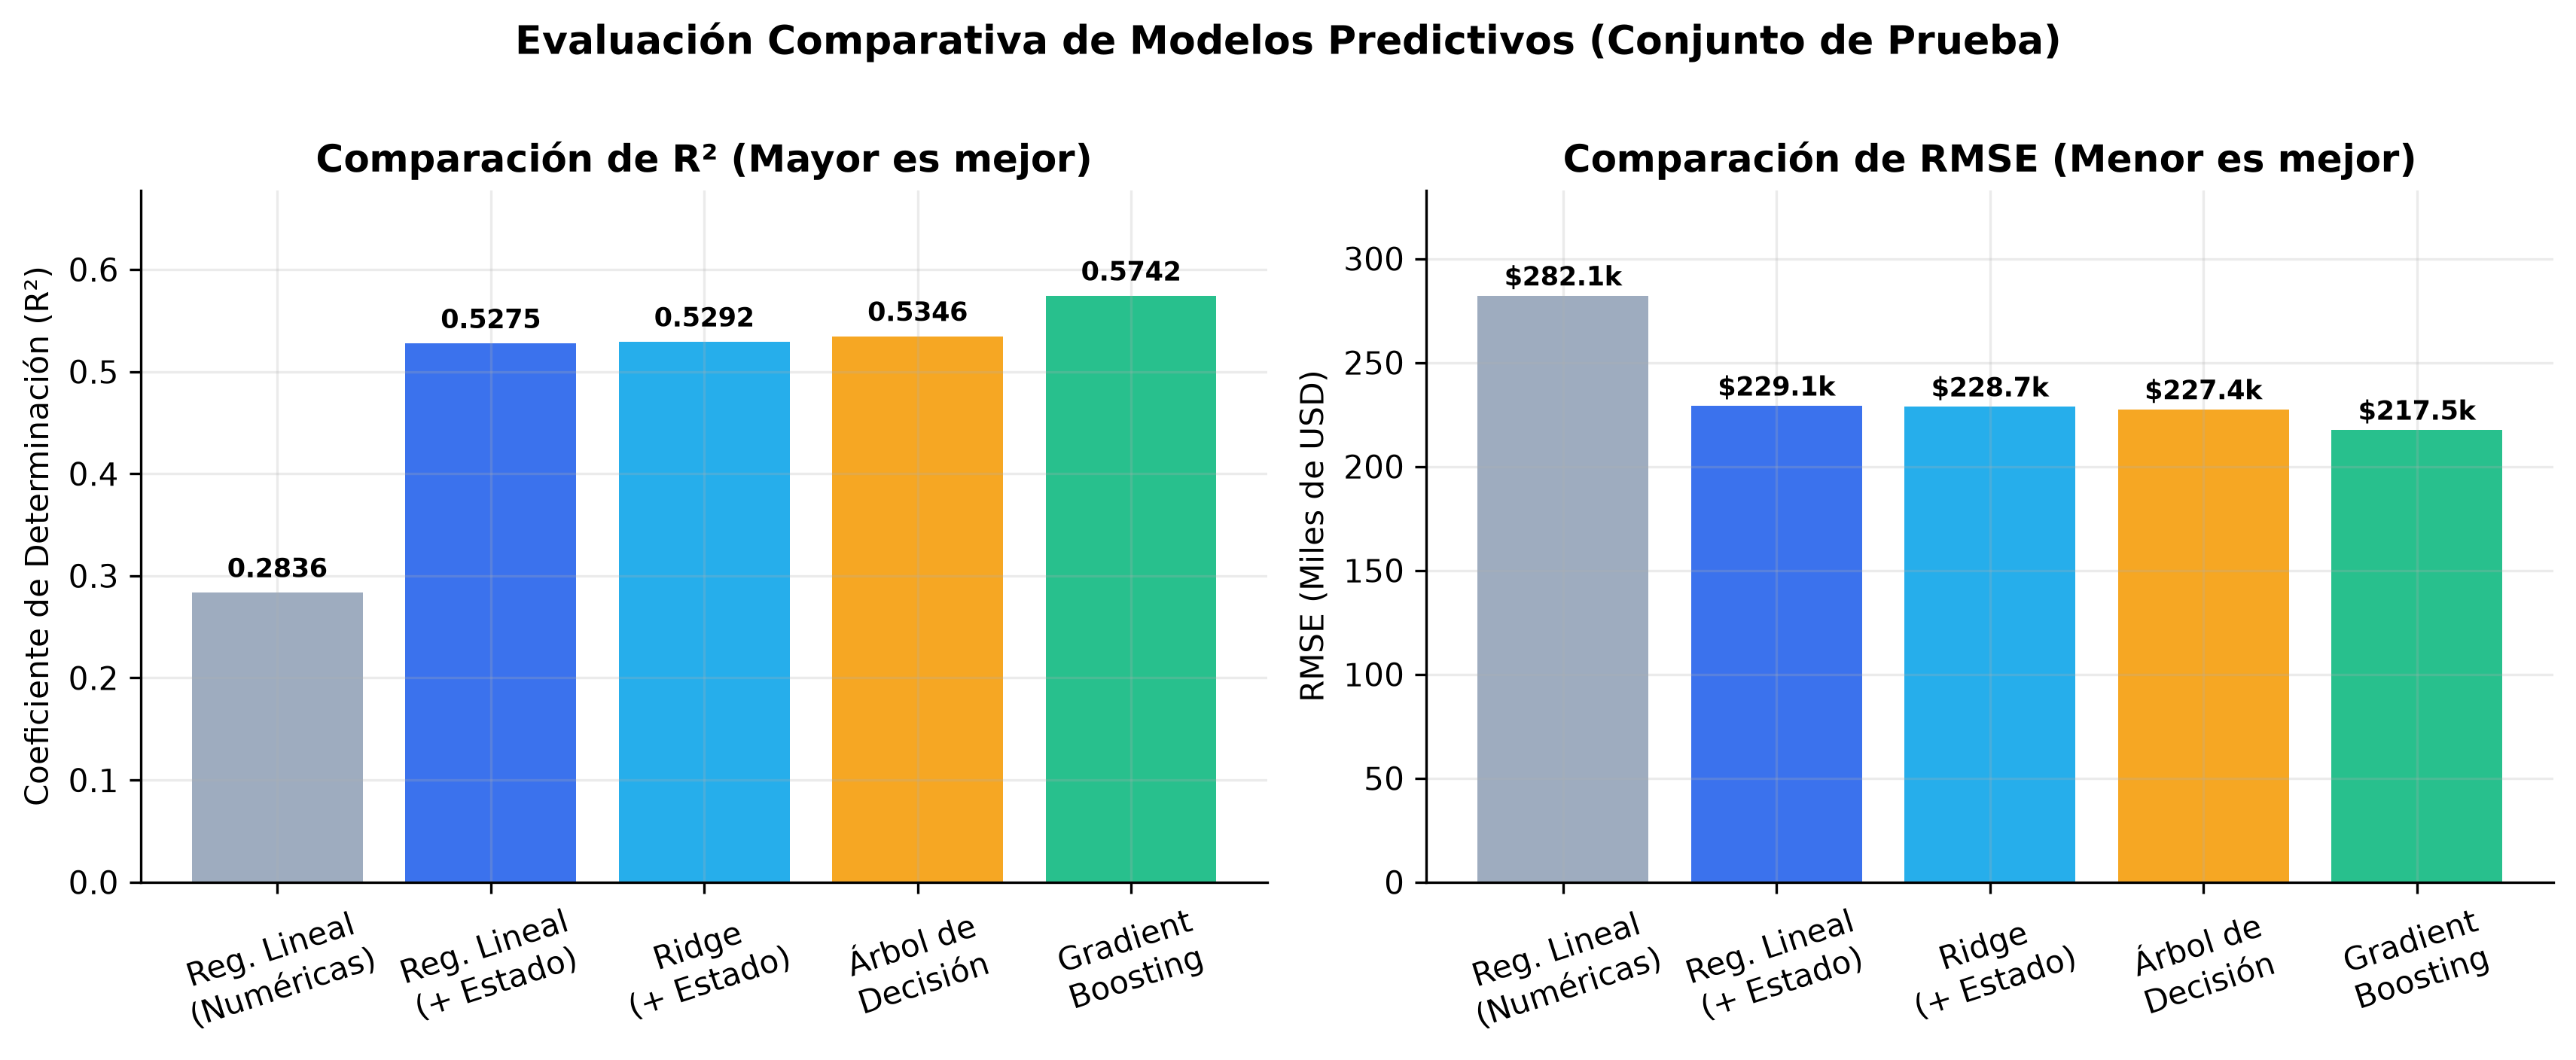
\includegraphics[width=0.95\textwidth]{figuras/comparacion_modelos.png}
    \caption{Comparación de $R^2$ y RMSE entre los cinco modelos evaluados.}
    \label{fig:comparacion}
\end{figure}

\subsection{Análisis de Resultados y Diagnóstico de Residuos}
De la Tabla~\ref{tab:modelos} y la Figura~\ref{fig:comparacion} se concluye que:
\begin{itemize}
    \item La incorporación del estado en la Regresión Lineal produce el salto más importante en desempeño: $+0.2439$ puntos en $R^2$ (de $0.2836$ a $0.5275$) y una reducción del error RMSE de casi \$53{,}000 USD.
    \item La Regresión Ridge ofrece resultados prácticamente equivalentes a la Regresión Lineal ordinaria ($R^2 = 0.5292$), confirmando que dado el gran tamaño muestral ($>1$ millón de registros), la varianza de los coeficientes lineales es muy baja.
    \item \texttt{HistGradientBoostingRegressor} obtiene el mejor ajuste global ($R^2 = 0.5742$, MAE = \$141{,}120 USD) al capturar interacciones no lineales entre el estado y la superficie construida (por ejemplo, el precio por pie cuadrado en California es muy distinto al de Ohio).
    \item Sin embargo, la \textbf{Regresión Lineal (+ Estado)} ofrece una excelente relación entre simplicidad, transparencia matemática, velocidad de inferencia y tamaño de archivo (2.2 KB), por lo que resulta idónea para el simulador interactivo de esta práctica.
\end{itemize}

La Figura~\ref{fig:residuos} muestra la relación entre precios reales y predichos, así como la distribución de residuos centrada en cero, con mayor dispersión en propiedades de alto valor ($>\$1{,}000{,}000$ USD), lo cual evidencia heterocedasticidad moderada esperable al no contar con variables de nivel vecindario (\texttt{zip\_code} o acabados).

\begin{figure}[H]
    \centering
    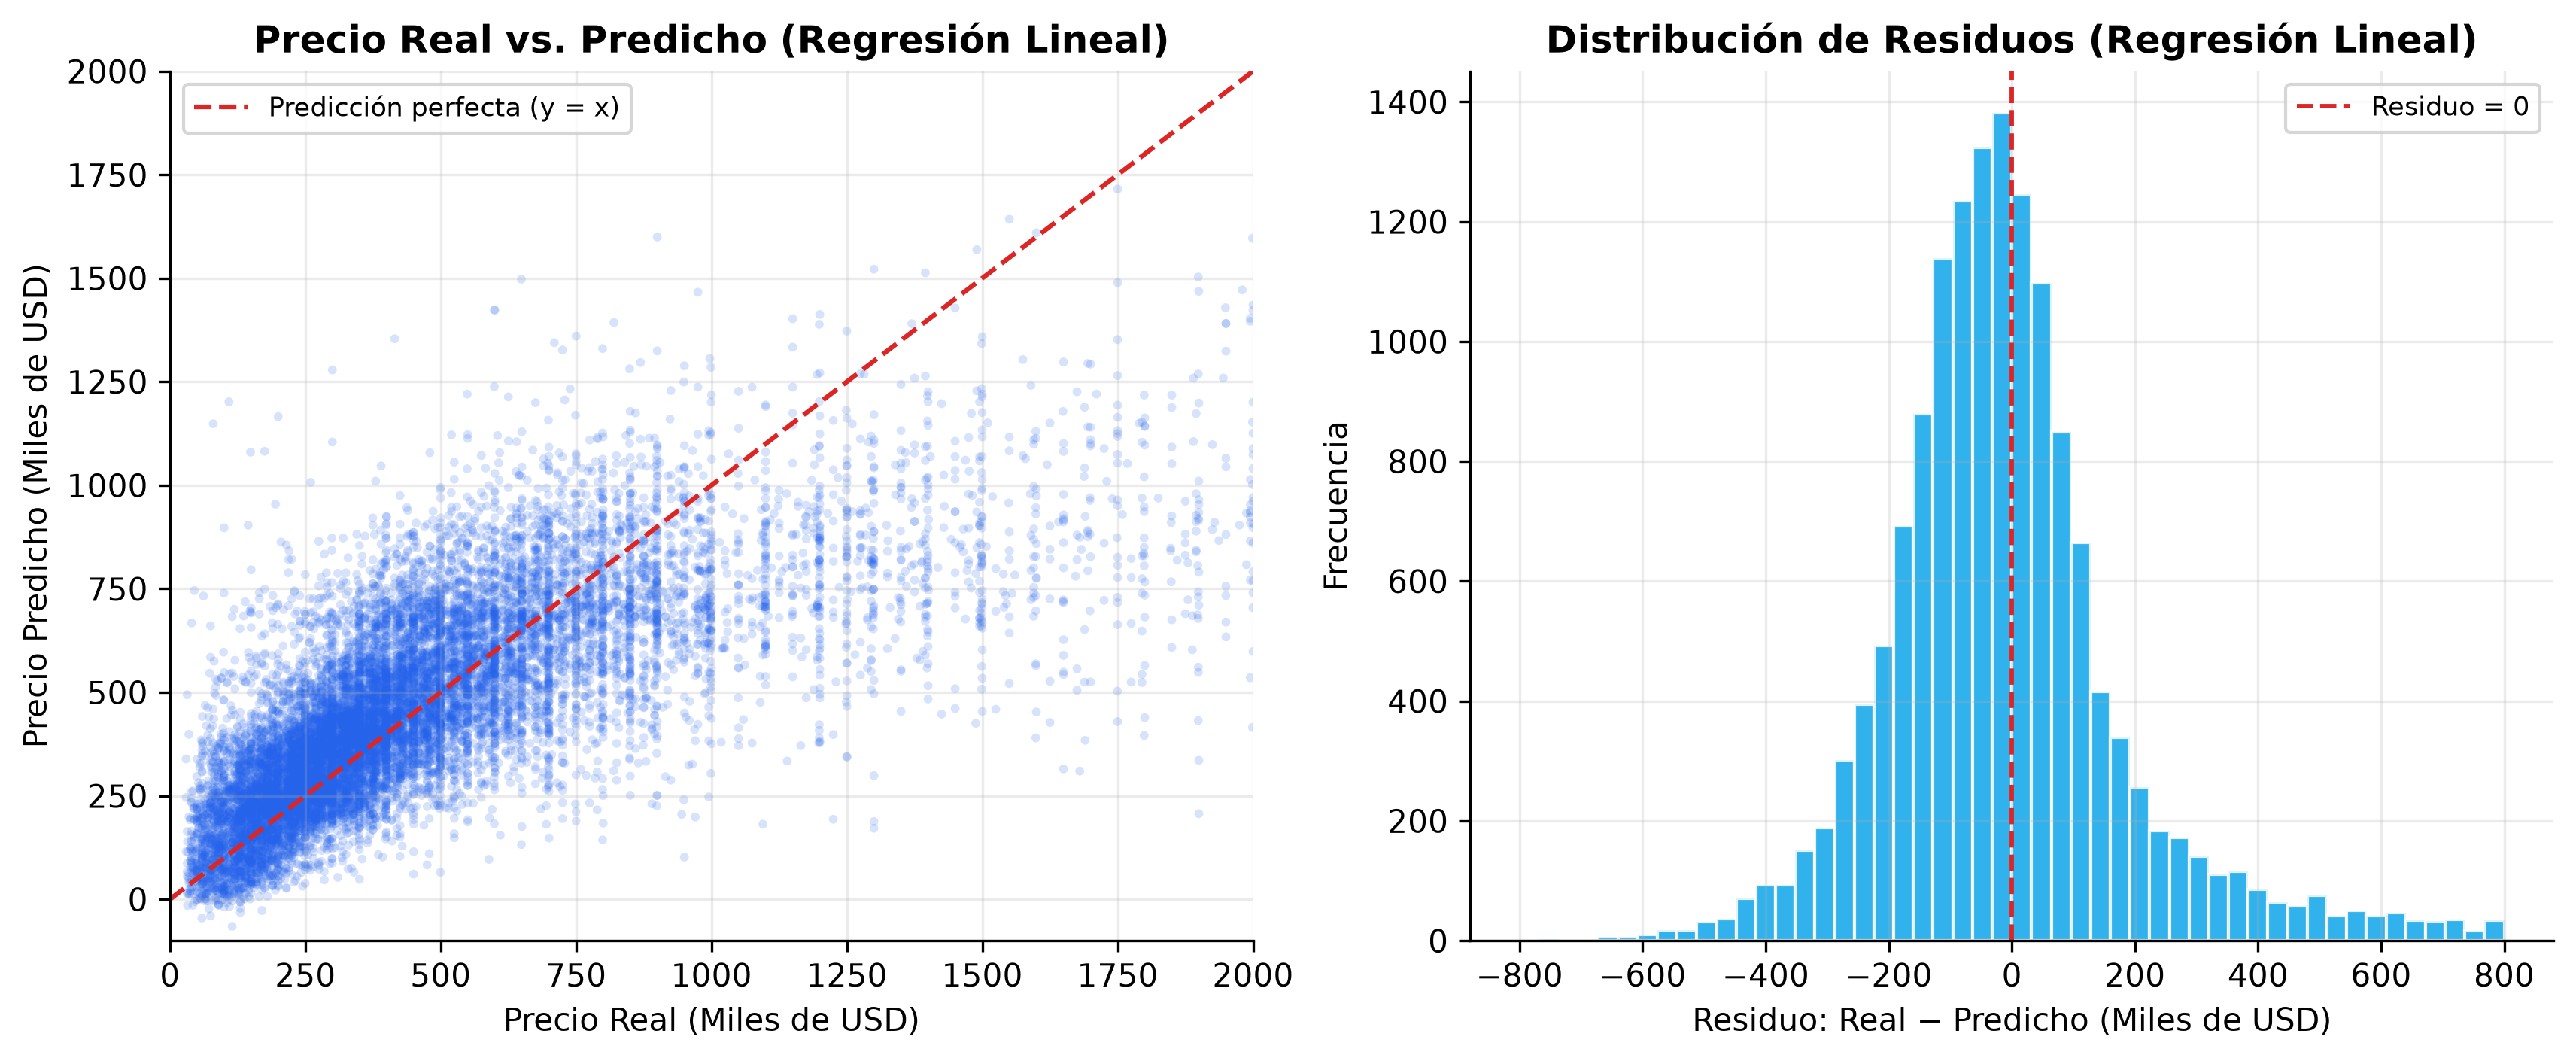
\includegraphics[width=0.95\textwidth]{figuras/real_vs_predicho.png}
    \caption{Diagnóstico del modelo de Regresión Lineal: valores reales vs. predichos y distribución de residuos.}
    \label{fig:residuos}
\end{figure}

\section{Visualización de Resultados y Simulador en Streamlit}

Para la presentación interactiva de resultados se desarrolló la aplicación web \texttt{app.py} en \textbf{Streamlit}, diseñada para despliegue directo en Streamlit Community Cloud. La aplicación incluye tres pestañas:
\begin{enumerate}
    \item \textbf{Simulador de Precio (Regresión Lineal):} Permite al usuario seleccionar el estado, la superficie construida (con soporte tanto en $\text{m}^2$ como en $\text{ft}^2$), número de habitaciones, baños y tamaño del terreno en acres. Al instante calcula el precio estimado mediante el modelo \texttt{LinearRegression} serializado (\texttt{models/linear\_regression\_model.joblib}), lo compara contra la mediana del estado y grafica la contribución individual de cada término de la ecuación lineal.
    \item \textbf{Análisis Exploratorio (EDA):} Presenta los indicadores clave del dataset, tabla de estadísticas descriptivas, matriz de correlación, histogramas interactivos y los 15 estados con mayor precio mediano.
    \item \textbf{Evaluación y Comparación de Modelos:} Muestra la tabla comparativa con MSE, RMSE, MAE y $R^2$, gráficas de desempeño, dispersión real vs. predicho y la interpretación de los coeficientes lineales.
\end{enumerate}

\section{Hallazgos, Limitaciones y Recomendaciones}

\subsection{Hallazgos Principales}
\begin{itemize}
    \item El tamaño construido (\texttt{house\_size}) y el número de baños (\texttt{bath}) son los principales impulsores físicos del precio residencial.
    \item La ubicación geográfica (\texttt{state}) explica casi la mitad de la varianza capturada por el modelo lineal, elevando $R^2$ de $0.2836$ a $0.5275$.
    \item Los modelos basados en ensambles de árboles (\texttt{HistGradientBoostingRegressor}) mejoran en $+0.0467$ puntos de $R^2$ respecto al modelo lineal al modelar interacciones entre ubicación y tamaño.
\end{itemize}

\subsection{Limitaciones y Recomendaciones}
\begin{itemize}
    \item \textbf{Granularidad geográfica:} Incorporar el código postal (\texttt{zip\_code}) o la ciudad mediante codificación por objetivo (\textit{target encoding}) permitiría capturar diferencias intraestatales (por ejemplo, Manhattan frente al norte del estado de Nueva York).
    \item \textbf{Variables del entorno:} En futuras iteraciones se recomienda enriquecer el dataset con indicadores socioeconómicos por código postal (ingreso mediano, calidad escolar, índice de criminalidad y cercanía a transporte público).
    \item \textbf{Transformación de la variable objetivo:} Modelar $\log(\text{price})$ puede reducir la heterocedasticidad observada en viviendas de lujo y mejorar el error porcentual medio.
\end{itemize}

\section{Conclusiones}

Se cumplió satisfactoriamente con todas las fases del proyecto, desde la limpieza de más de 2.2 millones de registros hasta el análisis exploratorio, el modelado estadístico con Regresión Lineal en \texttt{scikit-learn}, la comparación con algoritmos de Machine Learning y la creación de una aplicación interactiva en Streamlit. El modelo de Regresión Lineal Múltiple con ubicación geográfica logró un desempeño sólido e interpretable ($R^2 = 0.5275$), constituyendo una base clara y transparente para el simulador de precios y dejando abierta la mejora hacia modelos no lineales y variables socioeconómicas de mayor granularidad.

\end{document}
